\chapter{The Haero Driver}
\labelchapter{driver}

The standalone driver program, \texttt{haero\_driver}, provides a simple way to
explore the capabilities of Haero. It's a simple single-column model with a
bundled one-dimensional dynamics package. With it, you can

\begin{itemize}
  \item run single-column aerosol simulations
  \item perform statistical analysis on ensembles consisting of several columns
  \item conduct time-step convergence studies to build confidence in Haero's
        mathematical algorithms and their implementations
  \item select specific aerosol processes and parametrizations to examine
        in isolation, to debug or verify a given algorithm
  \item study how the aerosol processes interact with one-dimensional dynamics
        and other simplified physical process representations
\end{itemize}

In this chapter we describe the driver and its capabilities. The input format
for the driver is based on YAML and is described in \refappendix{driver_input}.

\section{Column Dynamics}

We use a one-dimensional (vertical) atmosphere and tests of increasing complexity.

Let $z=z(a,t)$ denote the trajectory of the particle labeled $a$ that arrives at physical position $z$ at time $t$.
The label $a$ is the Lagrangian, or material, coordinate. 
Particle trajectories are defined by
\begin{equation}\label{eq:traj}
\deriv{z}{t}(a,t) = w(z(a,t),t),
\end{equation}
where $w(z,t)$ is the vertical velocity.  
In the following sections, it will be convenient to formulate \eqref{eq:traj} in terms of the geopotential $\phi(a,t) = gz(a,t)$, 
\begin{equation}\label{eq:geo_traj}
  \deriv{\phi}{t}(a,t) = gw\left(\frac{\phi(a,t)}{g},t\right).
\end{equation}


Adiabatic column dynamics are described by the 1D Euler equations for a moist atmosphere,
\begin{subequations}\label{eq:1d}
  \begin{align}
    \totd{w} &= -g\left(\frac{1}{\rho}\partd{p}{\phi} + 1\right), \label{eq:momentum}\\
    \totd{\rho} &= - g\rho \partd{w}{\phi}, \label{eq:continuity}\\
    \totd{\theta_v} &= 0, \label{eq:thermo},\\
    \totd{q_v} &= 0, \label{eq:qv}
  \end{align}
\end{subequations}
where $\rho$ is density, $p$ is pressure, $\theta_v$ is the virtual potential temperature, and $q_v$ is the water vapor mass mixing ratio.
As in \cite{Taylor2020}, we treat virtual potential temperature $\theta_v$ as a material invariant.
The momentum, continuity, thermodynamic equation, and transport equation (respectfully) combine with \eqref{eq:geo_traj} and the equation of state,
\begin{equation}\label{eq:eos}
  \frac{p}{\Pi} = \rho R \theta_v,
\end{equation}
to define the complete system.
Above, $\Pi = (p/p_{ref})^{\kappa}$ is the nondimensional Exner pressure, with constant $\kappa = R/c_p$, where $R$ is the dry air gas constant and $c_p$ is the specific heat of dry air at constant pressure.
We have 6 prognostic variables: $\phi, w, \rho, \theta_v, q_v, p$, and 6 equations in \eqref{eq:geo_traj}, \eqref{eq:1d}, \eqref{eq:eos}.
The boundary conditions are $w(0,t) = w(z_{top},t) = 0$.

The advantage of the Lagrangian frame of reference imposed by \eqref{eq:geo_traj} is that the material derivative becomes an ordinary time derivative, $D/Dt = d/dt$. 
Hence, for the remainder of this note we simply use $d/dt$ in our notation.

We begin with an ansatz that the velocity has a simple form,
\begin{equation}\label{eq:z_vel}
  w(z,t) = w_0\sin\frac{\pi z}{z_{top}}\sin \frac{2\pi t}{t_p},
\end{equation}
where we have introduced parameters for the maximum velocity, $w_0$, the top of the model column, $z_{top}$, and the period of oscillation $t_p$.  
This velocity satisfies the boundary conditions and the initial condition, $w(z,0) = 0$.
We assume that this velocity is valid for all time throughout the whole column, from $z=0$ to $z=z_{top}$.
In terms of the geopotential, \eqref{eq:z_vel} becomes,
\begin{equation}\label{eq:phi_vel}
  w(\phi,t) = w_0 \sin \frac{\pi \phi}{g z_{top}}\sin\frac{2\pi t}{t_p}.
\end{equation}
Since velocity is prescribed, it does not need to be prognosed. 
This eliminates \eqref{eq:momentum} from our system of equations \eqref{eq:1d}.
Our goal is to derive the other variables associated with 1D motion in a non-hydrostatic column so that we have consistent dynamics and thermodynamics.

Substituting \eqref{eq:phi_vel} in \eqref{eq:geo_traj} we discover a separable ODE,
\begin{align}
  \deriv{\phi}{t} &= gw_0\sin\frac{\pi \phi}{g z_{top}}\sin\frac{2\pi t}{t_p},\\
  \Rightarrow \int \csc\frac{\pi \phi}{g z_{top}}\,d\phi &= g w_0\int\sin\frac{2\pi t}{t_p}\,dt,
\end{align}
whose solution is
\begin{equation}\label{eq:phi_sol}
\phi(t) = \frac{2gz_{top}}{\pi}\arctan\left[\tan\frac{\pi \phi_0}{2g z_{top}}\exp\left(\frac{w_0t_p}{z_{top}} \sin^2 \frac{\pi t}{t_p}\right)\right].
  \end{equation}

\begin{figure}[H]
  \centering
  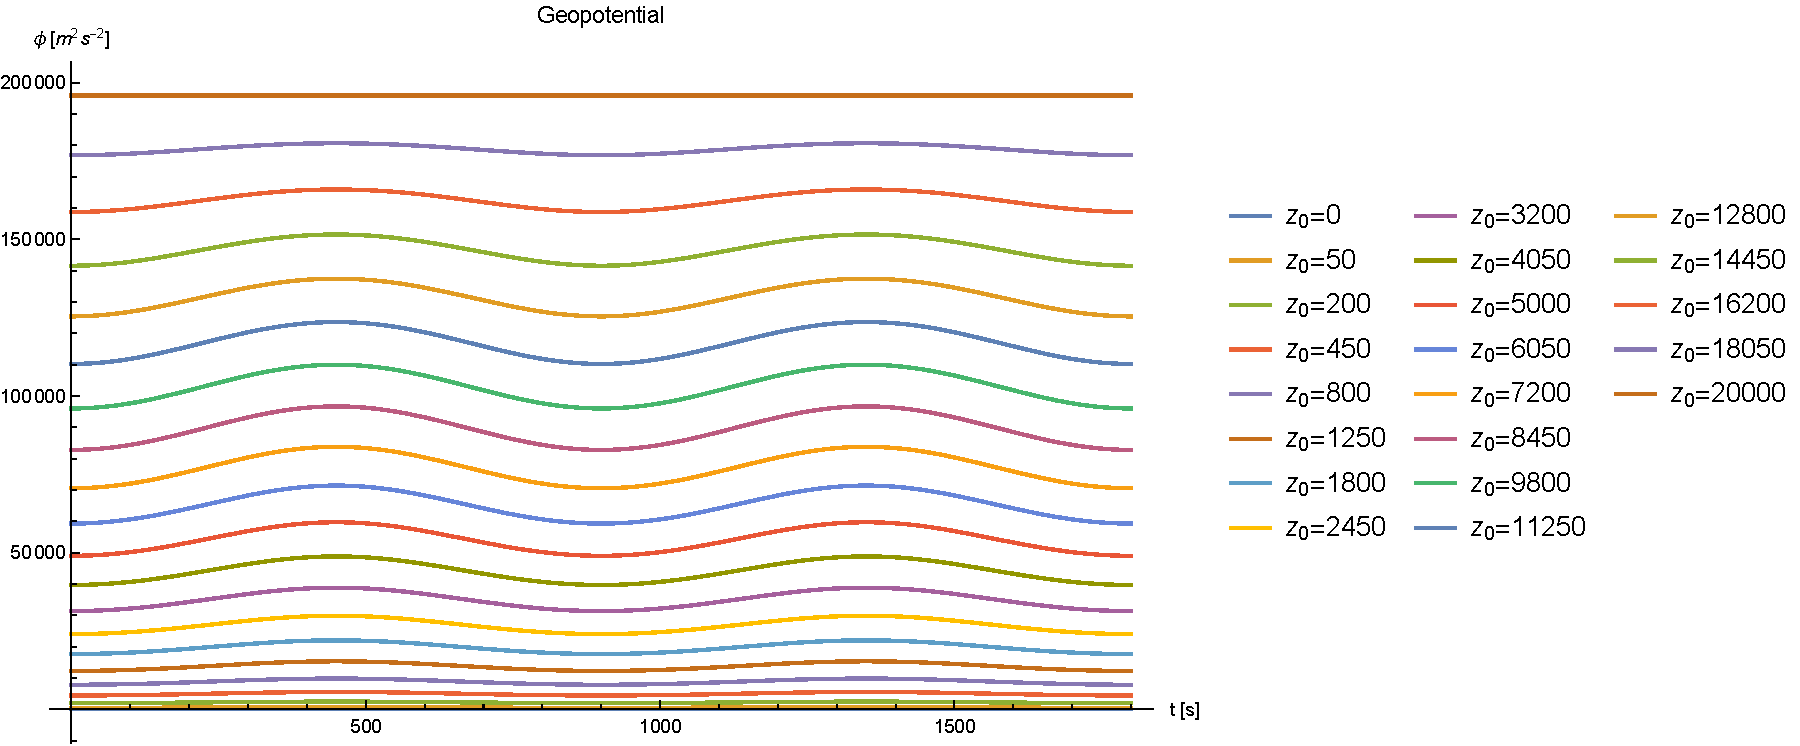
\includegraphics[width=\linewidth]{figures/geopotential_plot}
  \caption{Geopotential $\phi(t)$ for $\phi_0 = gz_0$ and $z_0$ values listed in the legend, with parameters $w_0=5$, $T_{v0}=300$, $\Gamma_v=0.01$, $z_{top}=20000$, $t_p=900$.}\label{fig:geopotential}
\end{figure}

We use \eqref{eq:phi_vel} to find the divergence, which is required by the continuity equation \eqref{eq:continuity},
\begin{equation}\label{eq:div}
  \partd{w}{\phi}(\phi,t) = \frac{\pi w_0}{g z_{top}}\cos\frac{\pi \phi(t)}{gz_{top}}\sin\frac{2\pi t}{t_p}.
\end{equation}
Substituting \eqref{eq:div} into \eqref{eq:continuity}, we find another separable ODE:
\begin{align*}
  \deriv{\rho}{t} &= -\rho \left(\frac{\pi w_0}{z_{top}}\cos\frac{\pi \phi(t)}{g z_{top}}\sin\frac{2\pi t}{t_p}\right)\\
  \Rightarrow \int \frac{1}{\rho}\,d\rho &= -\frac{\pi w_0}{z_{top}}\cos\frac{\pi \phi(t)}{z_{top}}\int \sin \frac{2\pi t}{t_p}\,dt.
\end{align*}
The solution is
\begin{align}\label{eq:density}
  \rho(\phi(t),t) = \rho_0(\phi_0)\exp\left[\frac{ w_0 t_p}{2z_{top}}\left(\cos\frac{\pi {\phi}(t)}{gz_{top}}\cos\frac{2\pi t}{t_p}-\cos\frac{\pi {\phi_0}}{gz_{top}}\right)\right].
\end{align} 

\begin{figure}[H]
  \centering
  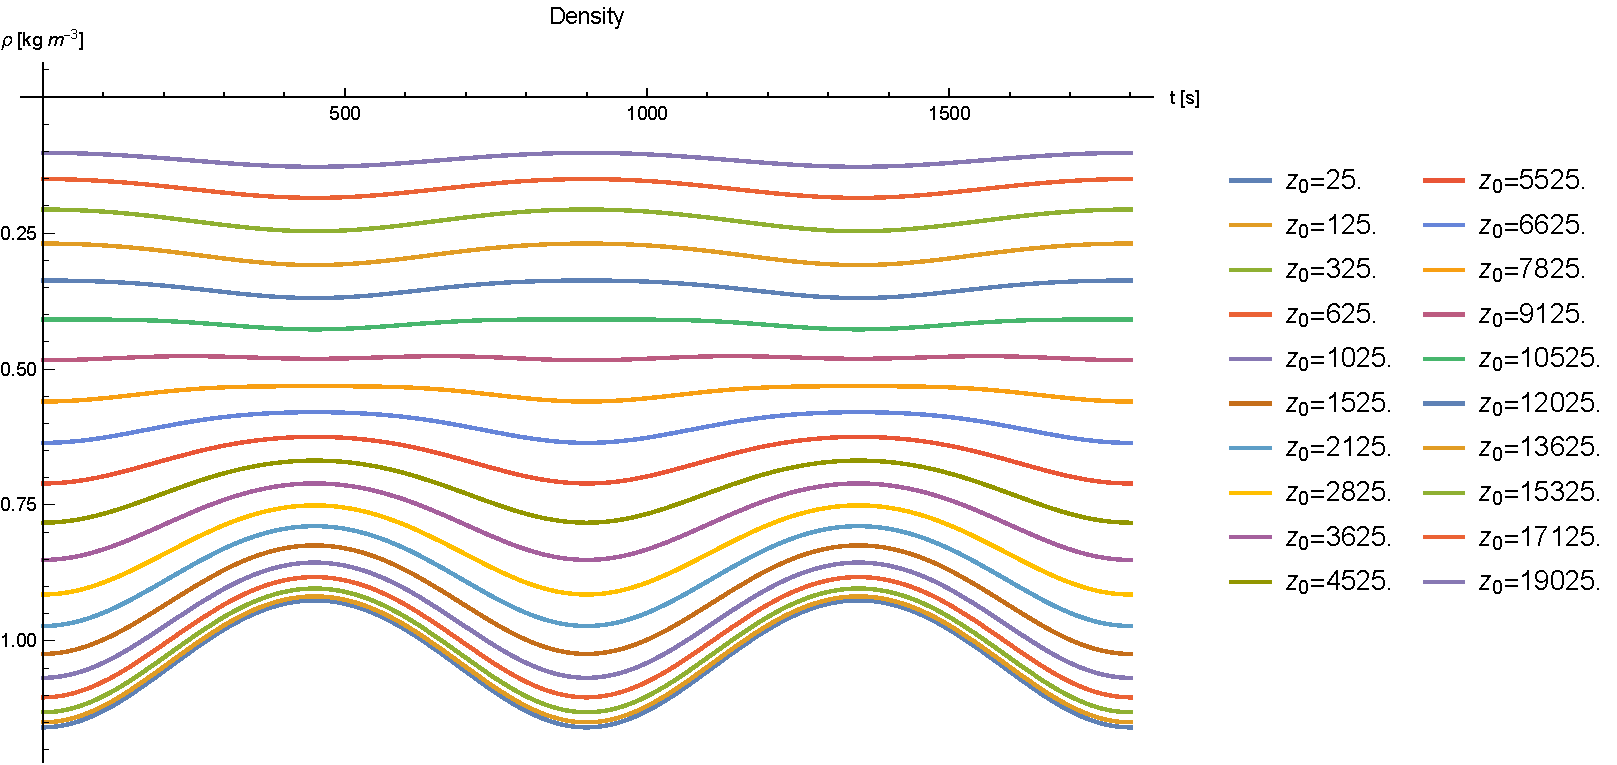
\includegraphics[width=\linewidth]{figures/density_plot}
  \caption{Density $\rho(\phi(t),t)$ for $\phi_0 = gz_0$ and $z_0$ values listed in the legend, with parameters $w_0=5$, $T_{v0}=300$, $\Gamma_v=0.01$, $z_{top}=20000$, $t_p=900$.}\label{fig:density}
\end{figure}

To find the pressure, we use \eqref{eq:density} in \eqref{eq:eos},
\begin{align}
  \frac{p}{\Pi} &= R\rho(\phi(t),t)\theta_v(\phi(t),t),\notag \\
  p(\phi(t),t) &= \left(p_{ref}^{-\kappa} R \rho(\phi(t),t)\theta_v(\phi(t),t)\right)^{1/(1-\kappa)}.\label{eq:pressure}
\end{align}

\begin{figure}[H]
  \centering
  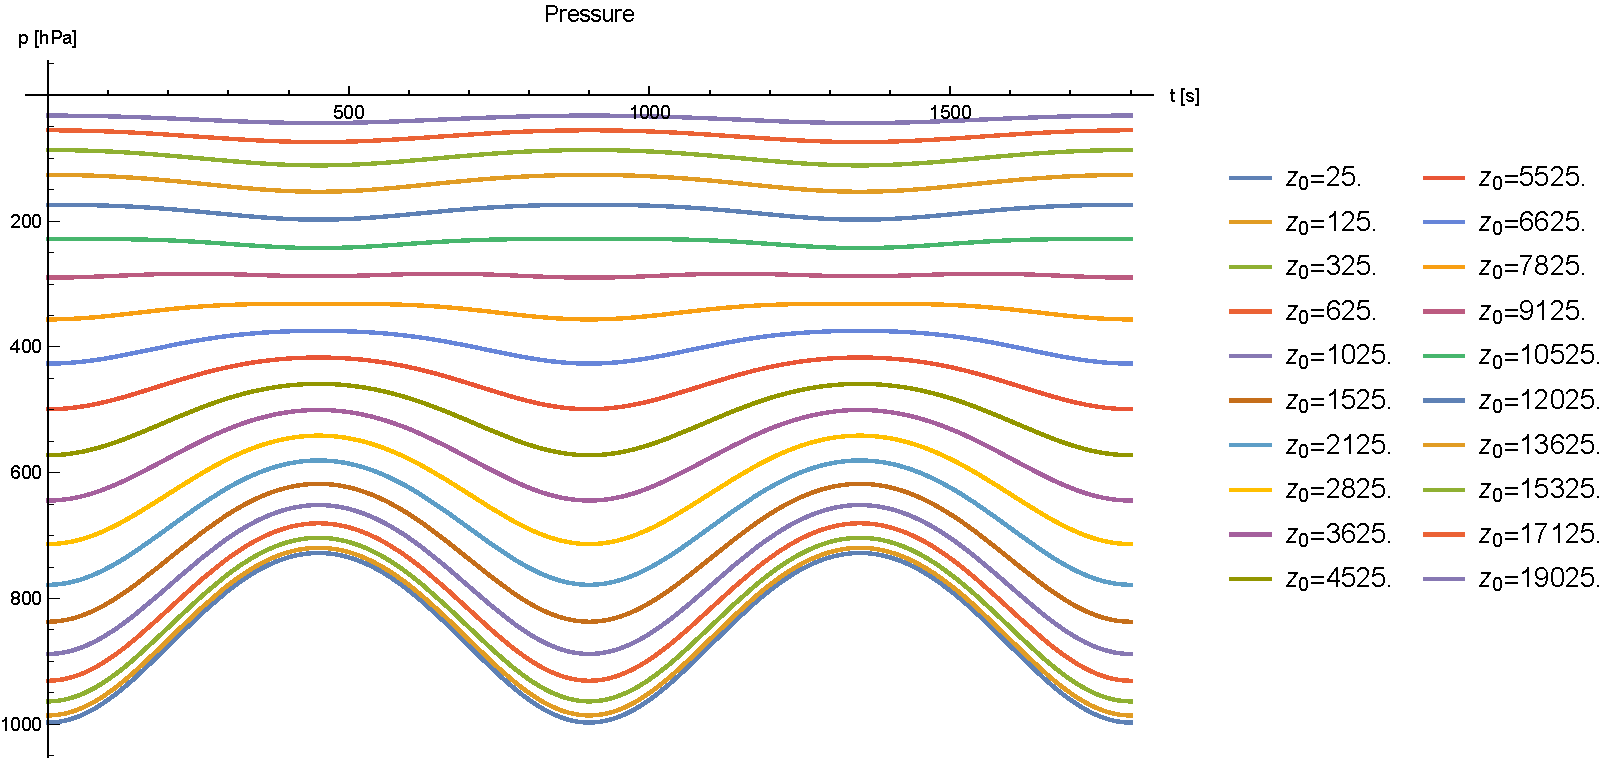
\includegraphics[width=\linewidth]{figures/pressure_plot}
  \caption{Pressure $p(\phi(t),t)$ for $\phi_0 = gz_0$ and $z_0$ values listed in the legend, with parameters $w_0=5$, $T_{v0}=300$, $\Gamma_v=0.01$, $z_{top}=20000$, $t_p=900$.}\label{fig:pressure}
\end{figure}

\subsection{Physical interpretation}

Physically, the ansatz \eqref{eq:z_vel} may be interpreted via \eqref{eq:momentum} as defining the balance between buoyancy, the pressure gradient force, and gravity to be,
\begin{align}
  -g\left(1 +  \frac{1}{\rho}\partd{p}{\phi}\right) &= \deriv{w}{t}(\phi,t), \notag \\
  &= \frac{2\pi w_0}{t_p}\sin\frac{\pi\phi}{gz_{top}}\cos\frac{2\pi t}{t_p} + \frac{\pi w_0^2}{2z_{top}}\sin\frac{2\pi\phi}{gz_{top}}\sin^2\frac{2\pi t}{t_p},
\end{align}
where the right-hand side is the time derivative of \eqref{eq:phi_vel}.
It is most straightforward to derive this interpretation by decomposing the pressure into a constant, hydrostatically balanced reference state with a superimposed perturbation \cite{KlempWilhelmson1978,Srivastava1967,SoongOgura1973} so that $p = \overline{p} + p'$.
Combining this decomposition (and similar treatment of temperature and density) with the equation of state leads to a formulation of the total pressure gradient as the background hydrostatic balance plus a perturbation due to nonhydrostatic buoyancy.  
In \cite{KlempWilhelmson1978,Srivastava1967,SoongOgura1973} this arises as quadratic terms of the perturbation variables are neglected.  
It is interesting that a similar (though not equivalent\footnote{Taylor et.~al.~\cite{Taylor2020} retain the full form of the pressure gradient, without a linearization.}) term arises in \cite{Taylor2020} as a result of the choice of a vertical mass coordinate based on hydrostatic pressure.
  
\subsection{Initialization}

Initial conditions are defined by stationary, $w(\phi(0),0) = 0,$ hydrostatic balance with a constant lapse rate in the virtual temperature profile, and exponential decay in the water vapor mixing ratio.

The initial virtual temperature profile is defined by two parameters, $T_{0}$ and $\Gamma_v$ (with default values 300K and 0.01 K/m, respectively),
\begin{equation}\label{eq:tv}
  T_{v0}(z) = T_{0} - \Gamma_v z.
\end{equation}
Using \eqref{eq:tv} with $p=\rho R T_v$, an equivalent form of the equation of state \eqref{eq:eos}, the hydrostatic equation $\partd{p}{z} = -\rho g$, and separation of variables (again), we derive expressions that relate initial height to initial pressure,
\begin{align}
  p_0(z) = \begin{cases}
          p_{ref}\exp\left(\frac{-g z}{R T_{0}}\right) & \Gamma_v = 0,\\[0.5em]
          p_{ref}\, T_0^{-g/(R\Gamma_v)}\left(T_{0} - \Gamma_v z\right)^{g/(R\Gamma_v)} & \Gamma_v \ne 0,
        \end{cases} \label{eq:p_of_z}\\[0.5em]
  z_0(p) = \begin{cases}
         -\frac{R T_{0}}{g}\log\frac{p}{p_{ref}} & \Gamma_v = 0,\\[0.5em]
         \frac{T_{0}}{\Gamma_v}\left(1 - \left(\frac{p}{p_{ref}}\right)^{R\Gamma_v/g}\right) & \Gamma \ne 0.
       \end{cases}\label{eq:z_of_p}
\end{align}
It follows that the initial virtual potential temperature profile is defined as
\begin{equation}
  \theta_{v0}(z) = T_{v0}(z)\left(\frac{p_{ref}}{p_0(z)}\right)^\kappa.
\end{equation}
The initial water vapor mixing ratio profile is also defined by two parameters, $q_0$ and $q_1$, with default values $q_0=0.015$ kg H$_2$O / kg air and $q_1 = $ 1E-3 m$^{-1}$, as
\begin{equation}\label{eq:init_qv}
  q_{v0}(z) = q_0e^{-q_1 z}.
\end{equation}
Initial densities are defined as
\begin{equation}
  \rho_0(z) = \frac{p_0(z)}{R\,T_{v0}(z)}.
\end{equation}

\subsection{Discretized column}

The Haero column is defined by first setting the required parameters using the \texttt{haero::driver::AtmosphericConditions} class.
These include the model top $z_{top}$, maximum vertical velocity $w_0$, and velocity period $t_p$ in \eqref{eq:phi_vel}, the initial virtual temperature profile \eqref{eq:tv}, and the initial water vapor mixing ratio profile \eqref{eq:init_qv}.

In the Haero driver, we emulate the vertical grid staggering used by the HOMME-NH dynamical core \cite{Taylor2020}, which has $n_{lev}$ levels and $n_{lev}+1$ interfaces.
Levels are indexed by integer values $k$, for $k=1,\dotsc,n_{lev}$ and interfaces are indexed by $k+1/2$, for $k=0,\dotsc,n_{lev}$.

In the \texttt{haero::driver::HostDynamics} class, geopotential and vertical velocity are defined at interfaces;
\begin{align}
  \phi_{k+1/2}(t) &= \frac{2gz_{top}}{\pi}\arctan\left[\tan\frac{\pi \phi_{k+1/2}(0)}{2g z_{top}}\exp\left(\frac{w_0t_p}{2z_{top}} \sin^2 \frac{2\pi t}{t_p}\right)\right], \label{eq:phi_disc}\\
  w_{k+1/2}(t) &= w_0 \sin \frac{\pi \phi_{k+1/2}(t)}{g z_{top}}\sin\frac{2\pi t}{t_p}. \label{eq:w_disc}
\end{align}
Similarly, density, virtual potential temperature, water vapor, and pressure are defined at level midpoints,
\begin{align}
  \rho_k(t) &= \rho_0(\overline{\phi_k}(0))\exp\left[\frac{ w_0 t_p}{2z_{top}}\left(\cos\frac{\pi \overline{\phi_k}(t)}{gz_{top}}\cos\frac{2\pi t}{t_p}-\cos\frac{\pi \overline{\phi_{k}}(0)}{gz_{top}}\right)\right], \label{eq:rho_disc}\\
  \theta_{vk}(t) &= \theta_{v0}(\overline{\phi_k}(0)/g), \label{eq:thetav_disc} \\
  q_{vk}(t) &= q_{v0}(\overline{\phi_k}(0)/g), \label{eq:qv_disc} \\
  % p_k(t) &= \left(p_0^{-\kappa}R \, \rho_k(t)\,\left(\theta_v\right)_k(t)\right)^{1/(1-\kappa)}, 
p_k(t) &=  \left(p_{ref}^{-\kappa} R \rho_k(t)\theta_{vk}(t)\right)^{1/(1-\kappa)}\label{eq:p_disc}
\end{align}
where the constants $g = 9.8$ m/s$^2$, $p_{ref} = 10^5$ Pa, and $\kappa = 0.286$; the overline denotes an average, $\overline{\phi_k}(t) = (\phi_{k-1/2}(t) + \phi_{k+1/2}(t))/2$.

Users may opt to initialize a column with uniform spacing in either height or pressure (at interfaces), or to specify their own height or pressure interfaces via an input \texttt{.yaml} file.  
The model top is defined by \eqref{eq:z_of_p}.  

Unit tests verify the expected 2nd order convergence of the centered finite difference methods used by both HOMME-NH and the Haero driver, and that layer thicknesses sum to the correct values $z_{top}$ and $p_{top}$, as shown in Figure \ref{fig:fd_verification}.

\begin{figure}[H]
\centering 
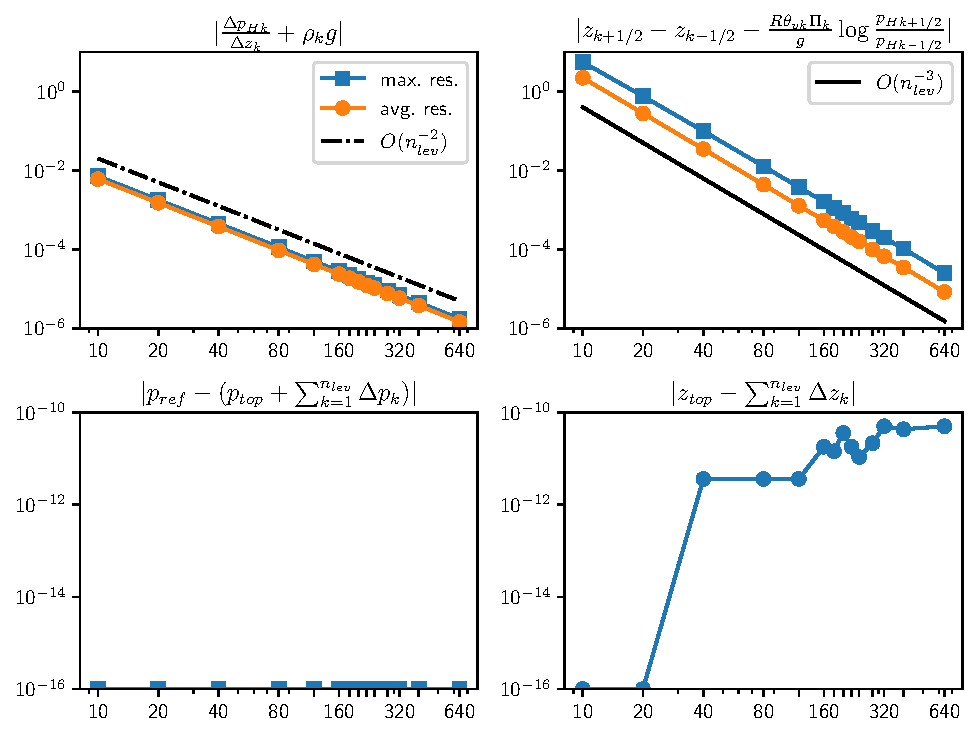
\includegraphics[width=0.8\linewidth]{figures/vconv_plot}
\caption{Vertical finite difference verification. Clockwise from top left: hydrostatic balance, hypsometric layer thickness, sum of height thicknesses, sum of pressure thicknesses.}\label{fig:fd_verification}
\end{figure}

\subsubsection{Layer thickness}

Layer thickness in height units is computed directly as 
\begin{equation}\label{eq:z_thick}
  \Delta z_k = \left(\phi_{k-1/2} - \phi_{k+1/2}\right)/g,
\end{equation}
which reflects the true thickness of a model level in our non-hydrostatic model.
However, some legacy parameterizations require thickness defined in \emph{pressure} units.
To support these parameterizations, we compute \texttt{hydrostatic\_dp} as a member of the \texttt{HostDynamics} class.
This calculation begins by defining the hydrostatic pressure $p_H$ at each interface, $p_{H,k+1/2} = p(\phi_{k+1/2}/g)$ using \eqref{eq:z_of_p}.
Then the layer thickness is computed as
\begin{equation}\label{eq:p_thick}
  \Delta p_{Hk} = p_{H,k+1/2} - p_{H,k-1/2}.
\end{equation}
\begin{assume}[Hyrdostatic layer thickness]
  Pressure thickness is computed via the hydrostatic approximation.  
\end{assume}

The interface hydrostatic pressures $p_H$ are stored as a private variable, to prevent users from mistaking them for the full non-hydrostatic pressure.

\subsection{Creating a Haero atmosphere}

The above dynamics are motivated by the input requirements of the various parameterizations.  
These are encapsulated by the \texttt{haero::Atmosphere} class, which requires temperature, pressure, height, and relative humidity data. 
We already have pressure and height.
Temperature may be diagnosed using the approximation given by \cite[eq.~(2.3)]{KlempWilhelmson1978},
\begin{equation}\label{eq:approx_temp}
  T_k(t) \approx \frac{\theta_{vk}(t) ~ \Pi_k(t)}{1+\alpha_q ~ q_{vk}(t)},
\end{equation}
with constant $\alpha_q = 0.61$.

\begin{figure}[H]
  \centering
  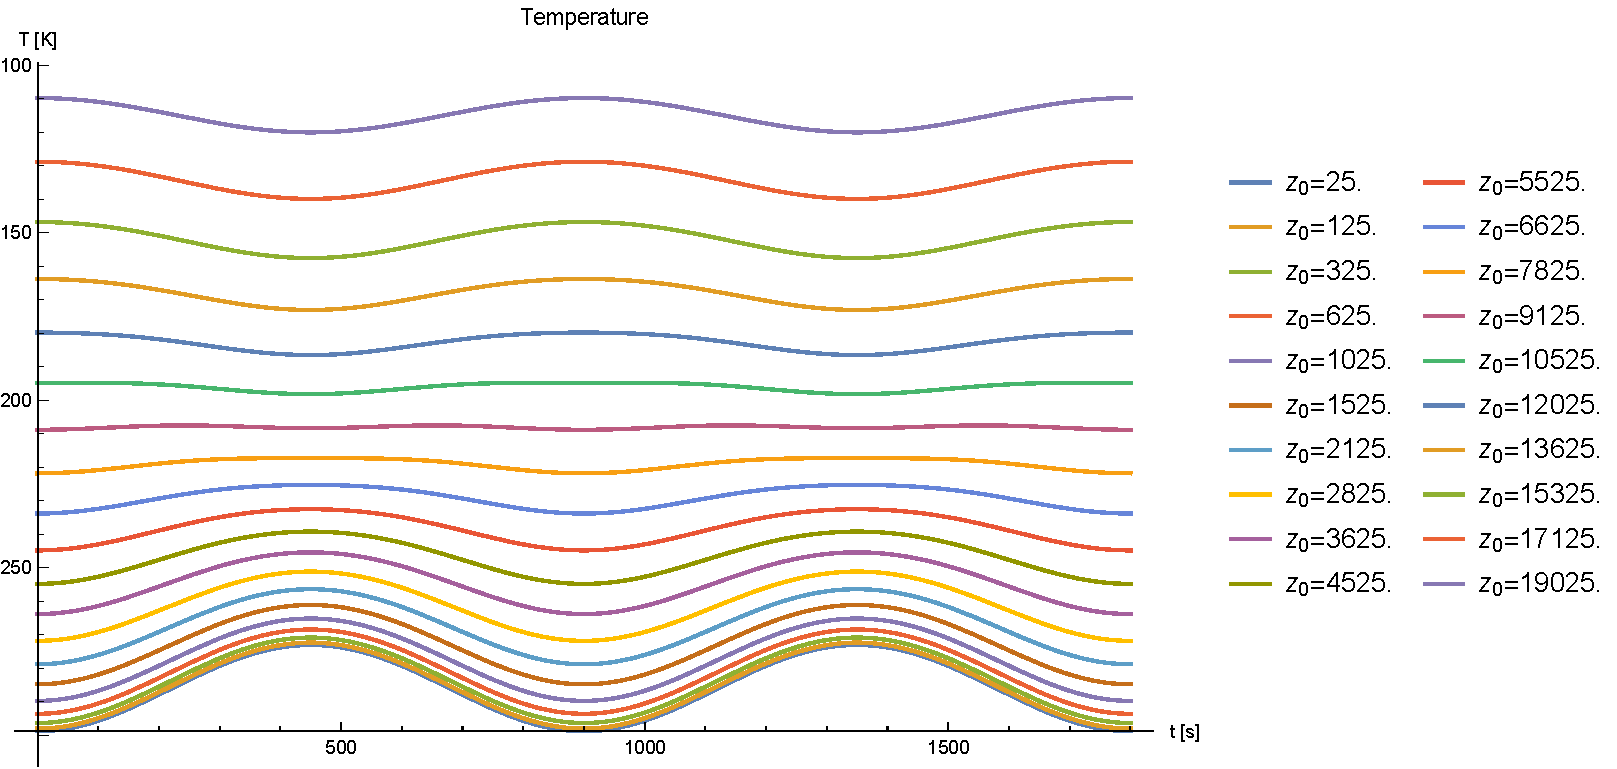
\includegraphics[width=\linewidth]{figures/temperature_plot}
  \caption{Temperature for the same parameters as in Figures \ref{fig:geopotential},\ref{fig:density}, and \ref{fig:pressure}, with the additional parameters $q_{0}=6$E-3, $q_1=2.5$E-3.}\label{fig:temperature}
\end{figure}

We compute relative humidity as $s = q_v/q_{vsat}$, where $q_{vsat}$ is the saturation mixing ratio.
We use the Tetens equation to find $q_{vsat}$ \cite[eqn. (A1)]{SoongOgura1973},
\begin{equation}\label{eq:tetens}
  q_{vs}(T) = \frac{380.042}{p}\exp\left(\frac{15}{2}\log(10) \frac{T-273}{T-36}\right).
\end{equation}

\begin{figure}[H]
\centering
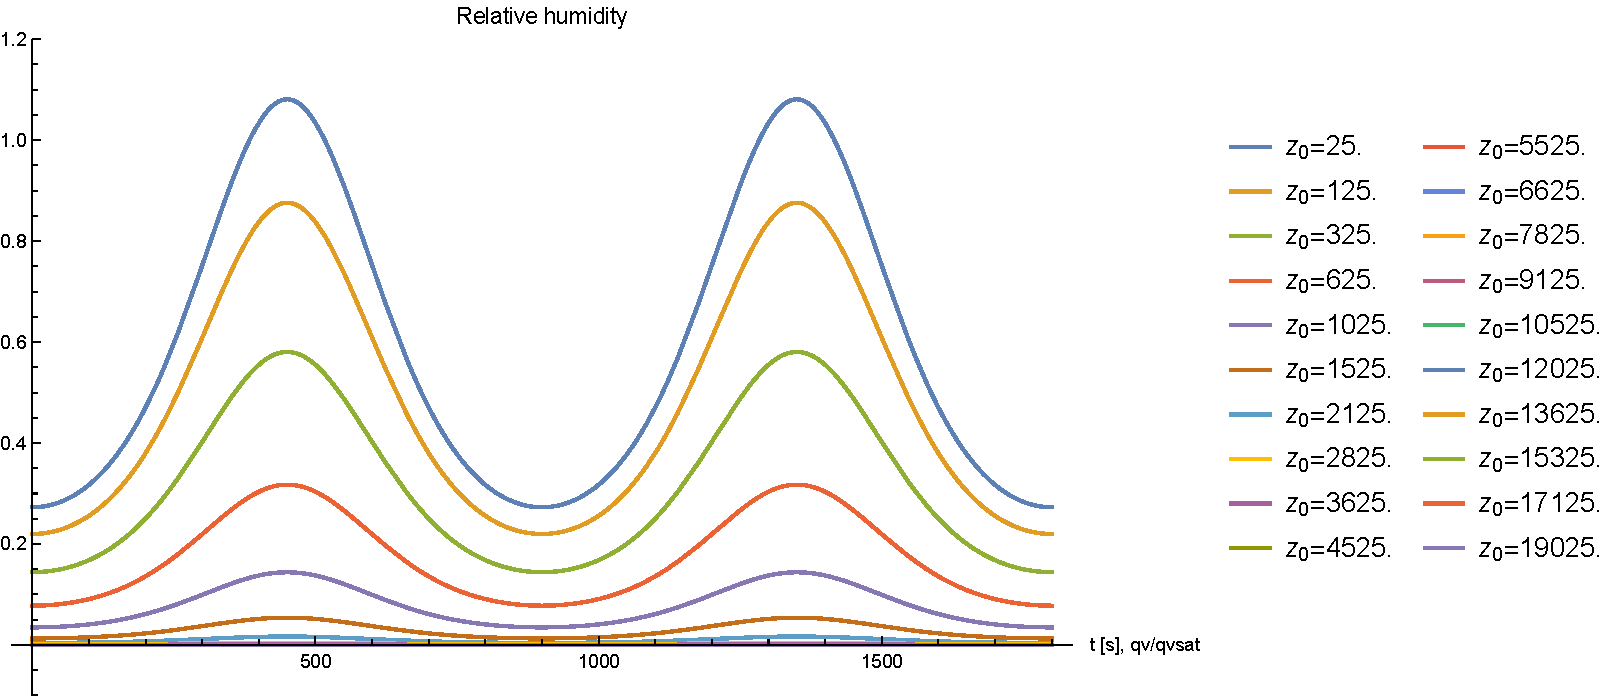
\includegraphics[width=\linewidth]{figures/relhumidity_plot}
\caption{Temperature for the same parameters as in Figures \ref{fig:geopotential},\ref{fig:density}, and \ref{fig:pressure}, with the additional parameters $q_{0}=6$E-3, $q_1=2.5$E-3.}\label{fig:humidity}
\end{figure}


\subsection{Time stepping}

The above dynamics are associated with the following \emph{tendencies}, the right-hand sides of \eqref{eq:geo_traj} and \eqref{eq:1d},
\begin{subequations}\label{eq:tends}
  \begin{align}
     \dot{w}(\phi,t) \equiv \totd{w}  &= \frac{2\pi w_0}{t_p}\sin\frac{\pi\phi}{gz_{top}}\cos\frac{2\pi t}{t_p} + \frac{\pi w_0^2}{2z_{top}}\sin\frac{2\pi\phi}{gz_{top}}\sin^2\frac{2\pi t}{t_p},\\
    \dot{\phi}(\phi,t) \equiv \totd{\phi} &= gw_0 \sin \frac{\pi \phi}{g z_{top}}\sin\frac{2\pi t}{t_p},\\
    \dot{\rho}(\phi, t, \rho) \equiv \totd{\rho} &= -\rho \frac{\pi w_0}{z_{top}}\cos\frac{\pi \phi}{g z_{top}}\sin\frac{2\pi t}{t_p},\\
    \dot{\theta_v} \equiv \totd{\theta_v} &= 0,\\
    \dot{q_v} \equiv \totd{q_v} &= 0,
  \end{align}
\end{subequations} 
where the dot denotes differentiation with respect to time.

\subsubsection{Simple microphysics}

A simple cloud model with warm-rain microphysics, often called \emph{Kessler microphysics}, is summarized in \cite[ch.~15]{RogersYau}, which references \cite{Srivastava1967}.
It introduces mass mixing ratio tracers for cloud liquid water $q_c$ and rain water $q_r$ and source terms for the dynamics equations.  
We use \cite{SoongOgura1973,KlempWilhelmson1978} as additional references.
We adapt this microphysics model here to match the HOMME-NH dynamics variables.

The two new tracers are advected passively by the dynamics (without source and sink terms) in the same manner as water vapor,
\begin{subequations}
  \begin{align}
    \dot{q_c} \equiv \deriv{q_c}{t} &= 0,\\
    \dot{q_r} \equiv \deriv{q_r}{t} &= 0.
  \end{align}
\end{subequations}
Microphysical parameterizations define approximate source and sink terms to correspond to a select (incomplete) set of physical processes, as described below.


\paragraph{Vertical velocity.} The vertical velocity $w$ is adjusted to account for loss of buoyancy due to the mass of suspended liquid water, 
\begin{equation*}
  \dot{w} \pluseq -g(q_c+q_r).  
\end{equation*}

\paragraph{Evaporation and condensation.}

Our first step assumes unsaturated air, $q_v \le q_{vs}$, where $q_{vs}$ is the saturation mixing ratio defined by \eqref{eq:tetens} using the temperature computed by \eqref{eq:approx_temp},
\begin{subequations}\label{eq:evap}
  \begin{align}
    \dot{q_v} &\pluseq E_{cv} + E_{rv}, \\
    \dot{q_c} &\minuseq E_{cv}, \\
    \dot{q_r} &\minuseq E_{rv},  \\
    \dot{\theta_v} &\minuseq \frac{L}{c_p \Pi}(E_{cv} + E_{rv}),
  \end{align}
where $E_{cv}$ and $E_{rv}$ denote the evaporation rates between cloud liquid/water vapor and rain/water vapor, respectively.
\begin{equation}\label{eq:cloud2vapor_evap}
   E_{cv} = \begin{cases} q_c & \text{if } q_v < q_{vs} \\ 0 & \text{otherwise}\end{cases}
\end{equation}
\begin{equation}
  E_{rv} = \begin{cases} \frac{(1-q_v/q_{vs}) C_{vt} (\rho q_r)^{0.525}}{\rho 5.4\text{E}5 + 4.1\text{E}6/e_s(T)} & \text{if } q_v < q_{vs} \text{ and } q_c = 0 \\ 0 & \text{otherwise}\end{cases}
\end{equation}
The ventillation coefficient $C_{vt} = 1.6 + 5.7\text{E-}2V_r^{3/2}$ for rain falling at speed $V_r$ relative to the air, and $e_s(T)$ is the saturation vapor pressure for a planar liquid water surface at temperature $T$.  
The latter two values are approximated as \cite[eqn.~(15))]{SoongOgura1973},
  \begin{align}
    V_r & = 36.34 (1\text{E}3\rho q_r)^{0.1346} \text{ m/s},\\
    e_s(T) & = 6.1094\exp\left( \frac{17.625 (T-273)}{T-29.96} \right)\text{ hPa}.
  \end{align}
\end{subequations}

A second step \cite[eqns.(A7)--(A10)]{SoongOgura1973} conducts an adjustment for supersaturated air, $q_v > q_{vs}$, after the time stepping procedure implied by \eqref{eq:evap} is finished.
Let these values be denoted by a star: $\theta_v^*$, $q_v^*$, $q_c^*$, etc. 
\begin{subequations}
Define the factor $r_1$,
\begin{equation}
  r_1 = \left(1 + \frac{237 a\Pi q_{vs}^*}{(T^*-36)^2}\frac{L}{c_p\Pi} \right)^{-1}.
\end{equation}
Then the adjusted values are given as
\begin{align}
  q_v &= q_{v}^* - r_1(q_v^*-q_{vs}^*),\\
  \theta_v & = \left(\theta^* + \frac{Lr_1}{c_p\Pi}(q_v^*-q_{vs}^*)\right)\left(1 + \alpha_v q_v\right),\\
  q_c &= q_v^* + q_c^* - q_v.
\end{align}
\end{subequations}


\paragraph{Autoconversion.} Autoconversion of cloud liquid into rain only occurs in the presence of sufficient cloud water droplets.
Here, ``sufficient'' is defined as greater than a constant critical value, $q_c^{(crit)}$, and \cite[eqn.~(12)]{Srivastava1967}
\begin{subequations} \label{eq:autoconversion}
\begin{align}
  \dot{q_c} &\minuseq \alpha_{auto}(q_c - q_c^{(crit)})_+,\\
  \dot{q_r} &\pluseq \alpha_{auto}(q_c - q_c^{(crit)})_+,
\end{align}
\end{subequations}
where $\alpha_{auto}$ [1/s] is the inverse of the autoconversion time scale and $q_c^{(crit)}$ is a user-defined parameter.
In \cite{SoongOgura1973}, $\alpha_{auto}=1\text{E-3}$ s$^{-1}$ and $q_c^{(crit)} = 1\text{E-3}$.

\paragraph{Accretion.} Accretion describes the capture of cloud water droplets by rainwater droplets.
As in \cite{SoongOgura1973,KlempWilhelmson1978}, we use
\begin{subequations}\label{eq:accretion}
\begin{align}
  \dot{q_c} &\minuseq \alpha_{accr}q_cq_r^{7/8}, \\
  \dot{q_r} &\pluseq \alpha_{accr} q_c q_r^{7/8},
\end{align}
\end{subequations}
with $\alpha_{accr} = 2.2$.

\paragraph{Rainwater sedimentation.} 

\begin{equation}
  \dot{q_r} \minuseq \frac{1}{\rho}\partd{}{z}(\rho V_rq_r)
\end{equation}

At the model top, this term is zero.

\todo{lower boundary}

\paragraph{Turbulent mixing.}

We modify sub-grid scale turbulence mode of \cite{KlempWilhelmson1978} to use a simple Smagorinsky turbulent eddy mixing coefficient,
\begin{equation}
  K_m = \sqrt{2}\left(\frac{7l}{50}\right)^2 \abs{\partd{w}{z}}.
\end{equation}
The additional source terms are \cite[eqns.~(3.15)--(3.16)]{KlempWilhelmson1978}
\begin{align}
  \dot{w} &\pluseq 2 \partd{}{z}\left(K_m \partd{w}{z}\right) - \frac{20}{3 l^2}K_m\partd{K_m}{z},\\
  \dot{q_v} &\pluseq 3\partd{}{z}\left(K_m\partd{q_v}{z}\right), \\
  \dot{q_c} &\pluseq 3\partd{}{z}\left(K_m\partd{q_c}{z}\right), \\
  \dot{\theta} &\pluseq 3\partd{}{z}\left(K_m\partd{\theta}{z}\right). 
\end{align}
\todo{Boundary conditions}
\subsection{Embedded parameterization}
